\section{Data collection}


\rThree{This project uses an open fMRI dataset from previous studies by the Kamitani lab~\cite{guohuashenDeepImageReconstruction2020,horikawaGenericDecodingSeen2017}. Details of the data collection process are provided below.}

\subsection{Subjects}
The data were collected from 5 healthy volunteers aged between 23 and 33 years (4 males and 1 female). All subjects provided informed consent before the experiment, with the study protocol having been reviewed and approved by the Ethics Committee of the Graduate School of Informatics at Kyoto University (approval no.: KUIS{-}EAR{-}2017{-}002). The subjects had normal or corrected-to-normal vision. \rThree{The recorded data of three of the participants is pubclicly available online~\cite{guohuashenDeepImageReconstruction2020}}.

\subsection{Experimental setup}
% Description of Deeprecon Dataset (quote Horikawa/Kamitani)
The experimental design for the current study was the same as that of Shen et al.~\cite{shenDeepImageReconstruction2019} (only the data from the image presentation experiment are used in this study). The public dataset of Shen et al.~\cite{ds001506:1.3.1} contains three of the five subjects that are used in the current study.  Two types of image presentation experiments were performed: training and testing. All stimuli were rear projected onto a screen in an MRI scanner bore with a luminance-calibrated liquid crystal display projector. The stimulus images were displayed at the screen center with a size of 12° $\times$ 12° of visual angle on a gray background. We asked subjects to fixate on the center of the images cued by a circle of 0.3° $\times$ 0.3° of visual angle. Each subject used a custom-molded bite bar and/or personalized headcase from CaseForge Inc.\ to reduce head motion during fMRI data collection. Multiple scanning sessions were performed to collect data for each subject. Multiple scanning sessions were performed to collect data for each subject. Each consecutive session took a maximum of 2 hours, with each run taking 6 to 8 min. The subjects were free to rest adequately between runs or to terminate the experiment at any time. Each image was flashed for 8 seconds at a frequency of 2 Hz, after which the average brain activation during the 8 seconds was calculated. This procedure was repeated 5 times for each image. The experimental design is described in detail in the original paper by Shen et al.~\cite{shenDeepImageReconstruction2019}. There were three different categories of images shown to the subjects: natural training images, natural test images and artificial shapes test images. \rOne{Since artificial shapes are only used as test images and never as train images, they will not always explicitly named as `test' images always in the following}. The selection of natural images was the same as that used in the experiment by Horikawa et al.~\cite{horikawaGenericDecodingSeen2017}. The dataset consists of 1200 images that were extracted from the ImageNet database~\cite{dengImageNetLargescaleHierarchical2009} for the training dataset and 50 images for the test dataset. It was ensured that the overlap between the categories of the training and test dataset was minimized, thus this \rThree{dataset named `Deeprecon'} has a considerably lower overlap between the training and test data than, for example, the popular NSD dataset~\cite{allenMassive7TFMRI2022,shirakawaSpuriousReconstructionBrain2024}. The artificial shapes test dataset consists of 40 images in which 5 different artificial shapes (the same shapes of the study by Miyawaki et al.~\cite{miyawakiVisualImageReconstruction2008}) are depicted in 4 different colors on a uniform gray background. Graphic~\ref{fig:datasets_train_art} shows a sample of the Train/Test and artificial shapes images. Since the Brain-Diffuser algorithm requires descriptions (captions) of the images in addition to the images, Shirakawa et al.~\cite{shirakawaSpuriousReconstructionBrain2024} used crowd-sourcing to collect 5 short captions for each image in the training and test datasets for the natural images. In addition, 5 captions were also created for each image in the test dataset of artificial shapes for this work.

\begin{figure}[ht]
    \centering
    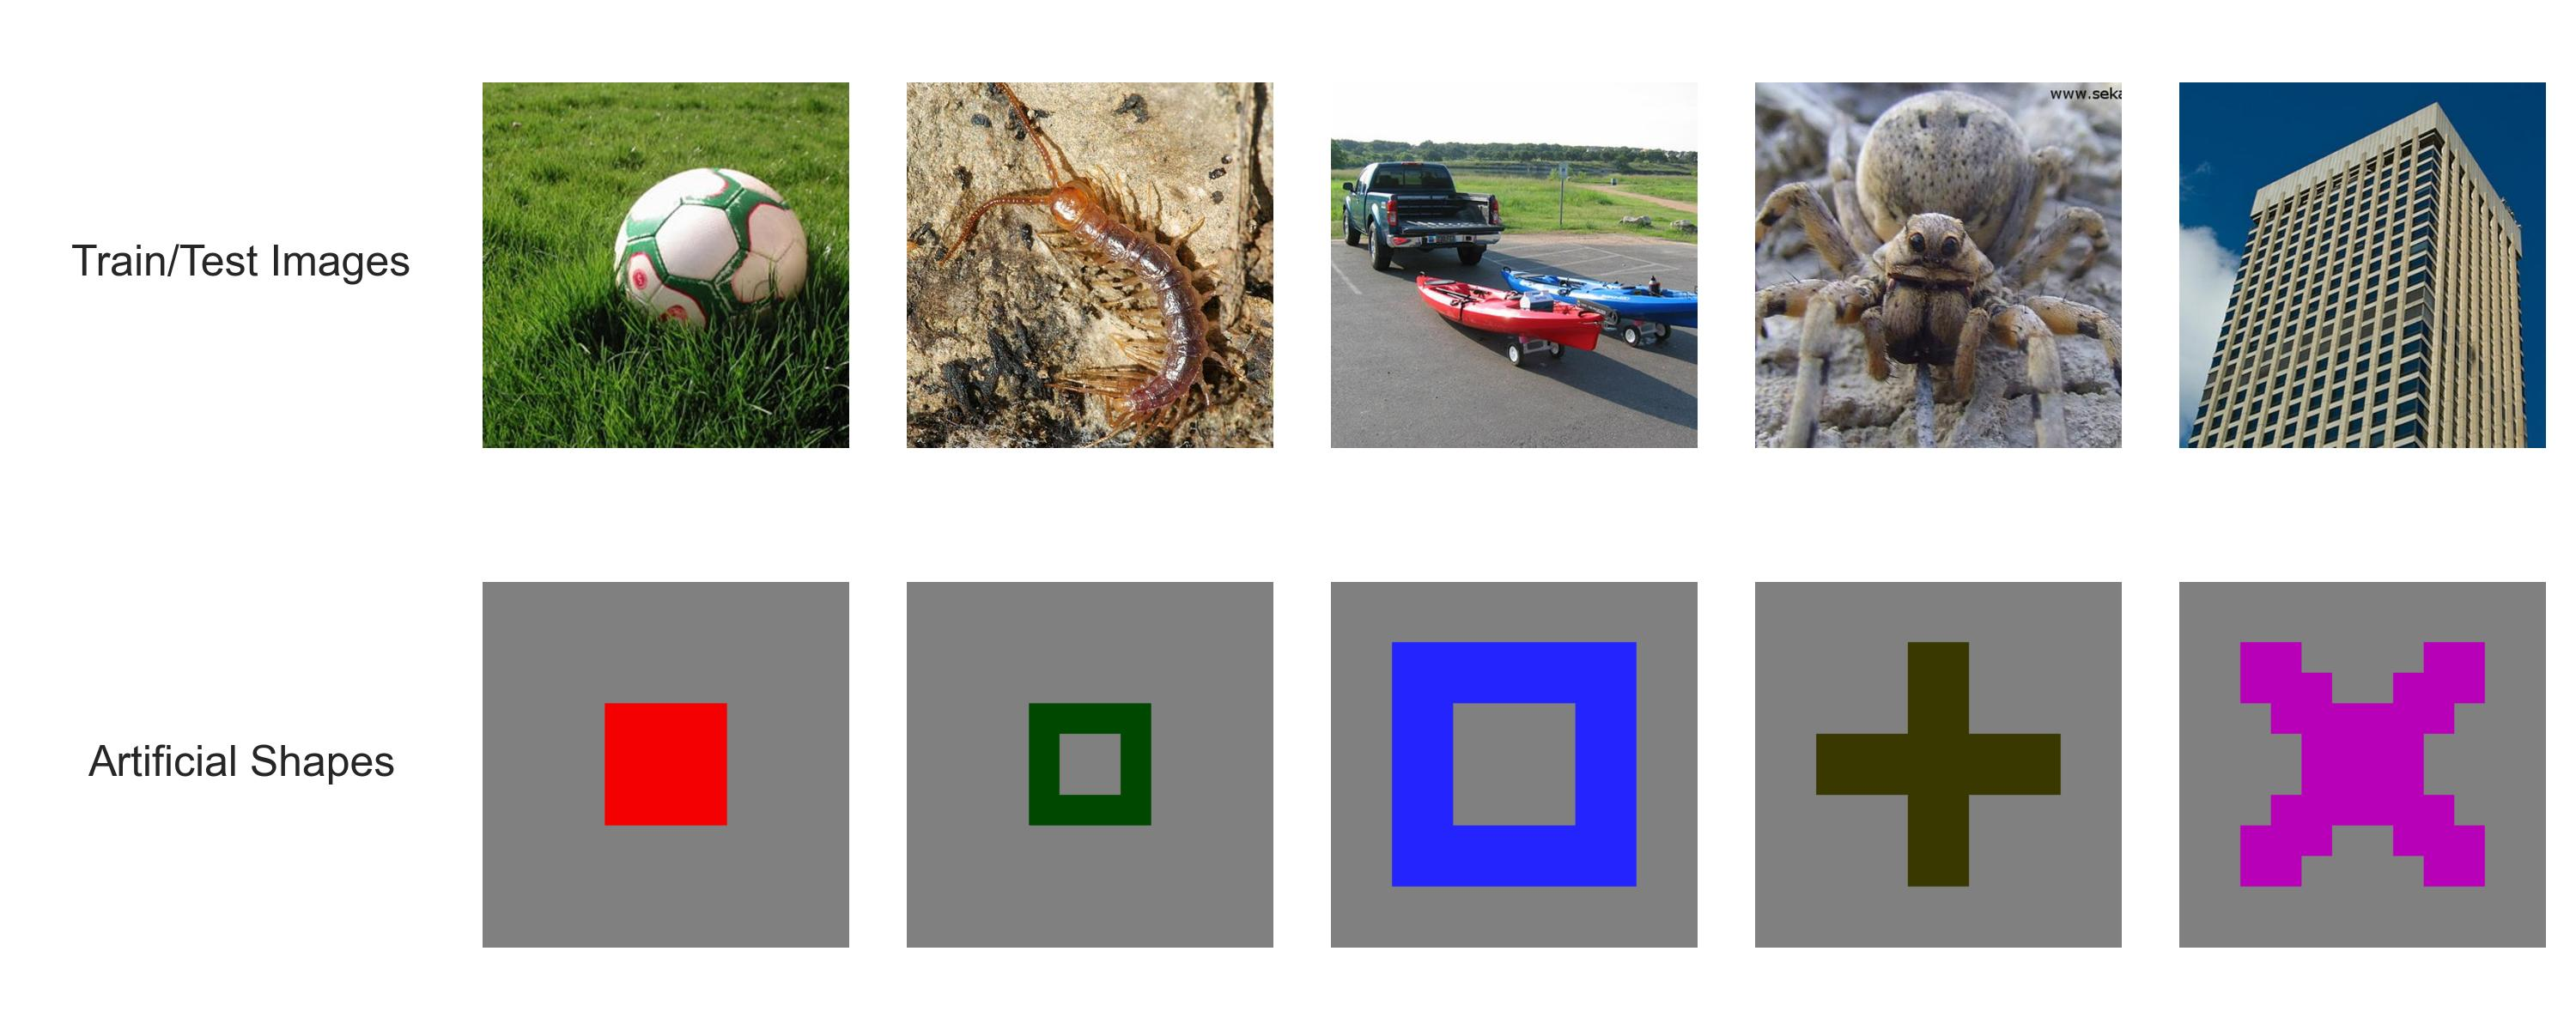
\includegraphics[width=0.8\textwidth]{plots/datasets_train_art_images.jpeg}
    \caption[Selection of natural images and artificial shapes]{\rOne{A selection of natural images (similar in the training dataset and the natural test images) and artificial shapes test images}}\label{fig:datasets_train_art}
\end{figure}

\subsection{MRI data}
% Hier kann ich evtl die Beschreibung aus dem Kamitani Lab nutzen
\subsubsection{MRI data acquisition}
The fMRI data was collected using a 3.0-T Siemens MAGNETOM Verio scanner at the Kyoto University Institute for the Future of Human Society (formerly, Kokoro Research Center). An interleaved T2*-weighted gradient-echo echo-planar imaging scan was performed to acquire functional images covering the entire brain [repetition time (TR), 2000 ms; echo time (TE), 43 ms; flip angle, 80°; field of view (FOV), 192 $\times$ 192 \rOne{mm\textsuperscript{2}}; voxel size, 2 $\times$ 2 $\times$ 2 mm3; slice gap, 0 mm; number of slices, 76; and multiband factor, 4]. T1-weighted (T1w) magnetization-prepared rapid acquisition gradient-echo fine-structural images of the entire head were also acquired [TR, 2250 ms; TE, 3.06 ms; inversion time (TI), 900 ms; flip angle, 9°; FOV, 256 $\times$ 256 \rOne{mm\textsuperscript{2}}; and voxel size, 1.0 $\times$ 1.0 $\times$ 1.0 \rOne{mm\textsuperscript{3}}].

\subsubsection{MRI data preprocessing}
MRI data preprocessing was performed through the pipeline of FMRIPREP (version 1.2.1). For the functional data of each run, a BOLD reference image was first estimated using a custom methodology of FMRIPREP.\@ Then, data were motion-corrected using MCFLIRT from FSL (version 5.0.9) and slice time-corrected using 3dTshift from AFNI (version 16.2.07), based on this BOLD reference image. Next, the corresponding T1w image was coregistered using boundary-based registration implemented by bbregister from FreeSurfer (version 6.0.1). The coregistered BOLD time-series were then resampled onto their original space (2 $\times$ 2 $\times$ 2 \rOne{mm\textsuperscript{3}} voxels) with antsApplyTransforms from ANTs (version 2.1.0) using Lanczos interpolation. After obtaining the resampled BOLD time series, the time series was first shifted by 4 s (two volumes) to compensate for hemodynamic delays, and then nuisance parameters from each voxel’s time series of each run were regressed out, including a constant baseline, a linear trend, and temporal components proportional to the six motion parameters calculated during the motion correction procedure (three rotations and three translations). Single-trial data samples were created by reducing extreme values (beyond ±3 SD for each run) of the time series and averaged within each 8 s trial (four volumes).

\subsubsection{Brain regions of interest}
According to standard retinotopy experiments~\cite{engelFMRIHumanVisual1994,serenoBordersMultipleVisual1995}, V1, V2, V3, and V4 were delineated. The LOC, FFA, and PPA were identified using conventional functional localizers~\cite{kanwisherFusiformFaceArea1997,epsteinCorticalRepresentationLocal1998,kourtziCorticalRegionsInvolved2000}. The higher visual cortex (HVC) region was defined by manually delineating a contiguous region that covered the LOC, FFA, and PPA on the flattened cortical surfaces. The VC was defined by combining V1 to V4 and the HVC.\@ For all the upcoming experiments, the whole VC was used for the reconstruction. After pre-processing the number of Voxels in the VC that can be used for the reconstruction task ranged from 13,135 to 16,667.

% {'S1': 13596, 'S2': 14597, 'S3': 13135, 'S4': 16067, 'S5': 13149, 'S6': 15316}

% Images were collected from an online image database ImageNet31 (2011, fall release), an image database where images are grouped according to the hierarchy in WordNet38. We selected 200 representative object categories (synsets) as stimuli in the visual image presentation experiment. After excluding images with a width or height o100 pixels or aspect ratio 41.5 or o2/3, all remaining images in ImageNet were cropped to the centre.

% Description of fmri-data 
%% Number of subjects
%% Number of runs per image
%% Experimental Design how the participants are shown the images
%% ROI Experiments
%% Chosen ROIs

\section{Reconstruction algorithms}

% How does the whole reconstruction pipeline look like? Both for iCNN and for Brain-Diffuser
In this work, the two algorithms Brain-Diffuser~\cite{ozcelikNaturalSceneReconstruction2023} and iCNN~\cite{shenDeepImageReconstruction2019}, that are described in more detail above, are used. The parameters for the algorithms that are used for this work are stated below. The entire codebase, which this work is based on, is publicly available on github~\cite{mildenbergerDiversity_thesis}, the associated README describes how to work with the codebase. 

\subsection{Brain-Diffuser}
% Brain-diffuser
Unless stated otherwise, the default settings described in the original publication are used for the Brain-Diffuser algorithm. For this purpose, the publicly available codebase~\cite{ozcelikOzcelikfuBraindiffuser2025} was used and adapted so that the Deeprecon data set can also be used.
First, the mean value of the measured brain activity of the 5 image presentations was calculated for each of the 1200 images in the training data set. This data serves as input for both the Brain-Diffuser algorithm and the iCNN algorithm. It should be noted that a better performance in the reconstruction could possibly result if the 5 presentations of each stimulus were included individually in the training data (i.e.\ a total of 6000 training samples are available). Since the main aim of this work is to investigate the relative difference between different test conditions and not to achieve the highest possible absolute performance, it was decided to calculate the mean value of the activation in order to save computing resources.

%% Regression
\subsubsection{Brain-Diffuser translator}
As is usual in reconstruction algorithms, the Brain-Diffuser algorithm first trains \rOne{translator} that map the brain activity into a latent space, which can then be used for reconstruction. There are three different \rOne{translators} that are trained for the Brain-Diffuser: one that maps the brain activity to the latent space of a VDVAE, one for CLIP Text features and one for the CLIP Vision features. The activations of all voxels recorded during the presentation of an image serve as predictor values.

The criteria to be predicted are the embeddings of the stimuli in the respective latent spaces of the three components. These true features must first be extracted from the simulus material. For the VDVAE, the model of Child et al.~\cite{childVeryDeepVAEs2020} is used, which was pre-trained with the ImageNet data set (64 $\times$ 64 pixels). As with the original Brain-Diffuser, only the first 31 layers of the total 75 layers of the VDVAE are used here, as adding further layers would not improve the prediction, but unnecessarily increase the size of the \rOne{translator} module. The 31 VDVAE layers of the embedded training images were concatenated so that the \rOne{translator} has to learn to predict a 91168-dimensional vector. 
Since CLIP~\cite{radfordLearningTransferableVisual2021} is a multimodal model, it can be used to extract both the true features from the presented images (CLIP Vision) and the associated captions (CLIP Text). For this work, a pre-trained CLIP network is used which is based on the Transformer architecture (ViT-L/14). For CLIP Vision, the images are embedded in a space with 257 $\times$ 768 values (256 image patches and a final vector for the entire image). For CLIP Text, the captions are embedded in a space with 77 $\times$ 768 values (76 tokens and a final vector for the entire caption). As 5 different captions were generated for each image, the average value of the latent space from all 5 captions is used as the true feature for CLIP Text.

% Ridge Regression

For the Brain-Diffuser algorithm, the linear ridge regression~\cite{hoerlRidgeRegressionBiased1970} is used for all \rOne{translators}. The ridge regression extends the linear regression by adding a penalty term, which is controlled via the coefficient $\lambda$ and regularizes (i.e.\ shrinks) the estimated coefficients. The higher $\lambda$, the more the parameters are shrunk. Especially in cases where a high dependency between individual predictors is to be expected, more robust parameters can be estimated in that way. Since the activation of neighboring neurons in the visual cortex is usually correlated~\cite{smithSpatialTemporalScales2008}, ridge regression is escpecially helpful in our case.

The ridge regression minimizes the following objective function:
\[
\min_{\beta} \sum_{i=1}^{n} {|y_i - x_i\top \beta|}^2 + \lambda |\beta|^2_F
\]
\noindent{}\rTwo{where \(y_i\) is the extracted \rOne{(true)} feature-vector (VDAVE, CLIP Text or CLIP Vision) for the \(i\)-train image or caption, \(x_i\) is the vector of recorded voxels in response to the \(i\)-th picture, \(\beta\) is the \rOne{matrix} of coefficients to be estimated, and \(\lambda\) is the regularization parameter controlling the strength of the penalty.} For the prediction of the latent space of the VDAVE, $\lambda_{\mathrm{VDVAE}}=50000$ is set, for CLIP Text $\lambda_{\mathrm{CLIP Text}}=100000$ and for CLIP Vision $\lambda_{\mathrm{CLIP Vision}}=60000$.


\subsubsection{Brain-Diffuser reconstruction}
% % Reconstruction
After the brain activity for the test datasets has been mapped to the latent spaces of VDVAE, CLIP Text and CLIP Vision using the \rOne{translators}, these \rOne{translated} features can be fed into the generator in the second step, which reconstructs the images.

% Versatile Diffusion
The Versatile Diffusion Algorithm~\cite{xuVersatileDiffusionText2024} is used as the reconstruction module in the Brain-Diffuser. The model used here was pre-trained on the Laion2B-en~\cite{schuhmannLAION400MOpenDataset2021} dataset. During the reconstruction itself, no parameters are trained, only the pre-trained parameters of the models are used. First, the generator part of the VDVAE is used to generate a first (blurry) approximation of the final reconstructed image from the predicted features. The VDVAE generates images with a size of 64 $\times$ 64 pixels, which are first scaled up to a size of 512 $\times$ 512 to serve as a prior for the Versatile Diffusion Generator. The image generated by the VDVAE adds noise to 37 of the 50 forward diffusion steps. In the backward-denoising process, the generated image is conditioned by both the predicted CLIP Vision (relative strength 0.6) and CLIP Text (relative strength 0.4) features. The generated images have a size of 512 $\times$ 512 pixels. \rThree{It should be noted, that the whole CLIP Vision and CLIP Text embeddings are used and not only the final output vector. Thus the dimensionality of the used CLIP Vision embeddings is 257$\times$768 (256 for all vision transformer patches in the image and one global CLIP vector) and 77$\times$768 for the CLIP Text embeddings (75 tokens and one global CLIP vector)}.

% iCNN
\subsection{iCNN}
Similarly to the brian-diffuser, the iCNN~\cite{shenDeepImageReconstruction2019} algorithm also consists of a \rOne{translator} and a reconstruction module. 
\subsubsection{iCNN \rOne{translator}}
The averaged activations of all voxels are again the predictors for the \rOne{translator}. The criteria are the features of a VGG19~\cite{simonyanVeryDeepConvolutional2014} model, with which the stimuli (resized to 224$\times$224 pixels) are encoded. The VGG19 implementation of PyTorch was used, whereby the weights of the Caffe implementation~\cite{ModelZoo} (pre-trained on ImageNet) were used to create the same conditions as in the original implementation by Shen et al.~\cite{shenDeepImageReconstruction2019}. The features from the 19 layers of the VGG were then reshaped into one-dimensional vectors. As with the Brain-Diffuser, a ridge regression is then also calculated, which predicts the features from the voxel data, the ridge parameter is set to $\lambda=50000$.

\subsubsection{iCNN reconstruction}
Once the brain activity of the test data sets has been mapped to the feature space of the VGG19 layer using the learned regression, the reconstruction of the images with the iCNN algorithm~\cite{shenDeepImageReconstruction2019} begins. First the predicted features ware scaled using the mean and standard deviation of the train images. The implementation of the BdPy package~\cite{KamitaniLabBdpy2024} is used for this (relu7 generator). The SGD optimizer is used and the number of iterations in which the reconstructed image is adapted to the predicted features is set to 500. Normally distributed noise was used as a prior.


\subsection{\rThree{Recovery check}}
\begin{figure}[ht]
    \centering
    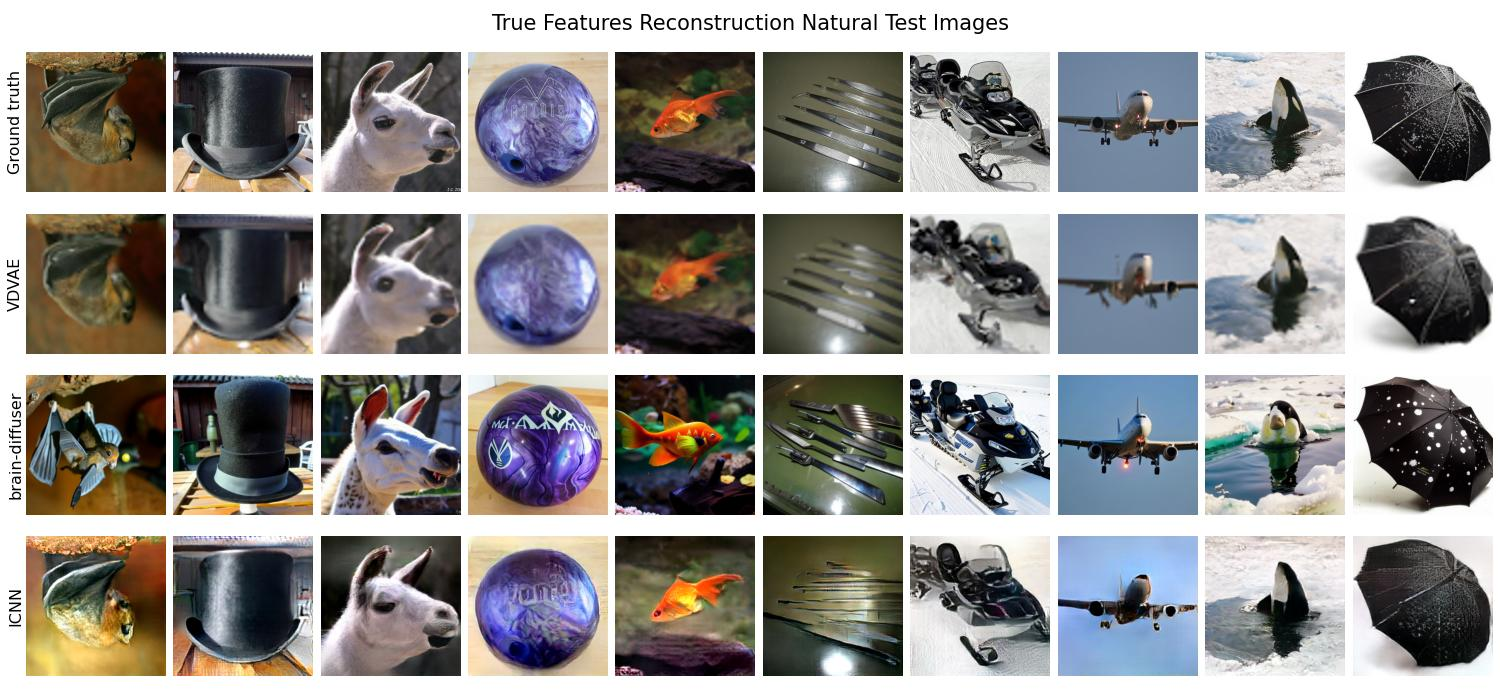
\includegraphics[width=1\textwidth]{plots/baseline_qual_true_recon_test.JPEG}
    \caption[Recovery check]{\rThree{Recovery check} reconstruction for natural test images. \rOne{The top row depicts the ground truth images. Each following row depicts the reconstruction with true features with the algorithm named on the left side.  Note that the VDVAE is only a part of the whole Brain-Diffuser algorithm.}}\label{fig:baselinetruerecon}
\end{figure}
\noindent{}\rOne{To \rThree{verify the} theoretical upper limit for the reconstruction performance of the two algorithms, the true features can be used for reconstruction. \rThree{This procedure is called `recovery check'.} Here, features extracted directly from the stimulus material are fed into the reconstruction module. This means that no brain data is used for the \rThree{recovery check}. It therefore offers the opportunity to see how good the reconstruction could be if the latent features could be perfectly predicted from the brain data.} Figure~\ref{fig:baselinetruerecon} \rOne{shows the recovery check for 10 of the 50 images of the test data set with natural images.}

\rOne{
In the figure, the \rThree{recovery check} is done both for the Brain-Diffuser (the intermediate result of the VDVAE and the final result of the versatile diffusion) and the iCNN algorithms. The first line shows the images that were presented to the test subjects during the experiment. In addition to the final result of the Brain-Diffuser algorithm (shown in the third row), the intermediate result of the VDVAE is also shown in the second row. It can be seen that the VDVAE algorithm shows a \rThree{precise} reconstruction performance for all images and is usually only a slightly blurred image of the ground truth. This is to be expected, as the VDVAE is precisely designed to reconstruct original images from a reduced feature space with as few errors as possible. The final result of the Versatile Diffusion of the Brain-Diffuser algorithm also shows \rThree{high} performance in principle, but it becomes apparent that details from the image are sometimes displayed incorrectly or are hallucinated. For example, the bat looks more like a bird, the fish swims in the wrong direction or additional writing is visible on the sphere. The iCNN algorithm is close to the result of the VDVAE.\ Most of the images can be displayed \rThree{with high quality}. However in particular, details and the coloring of backgrounds  are sometimes incorrectly reconstructed by the iCNN.}
% True-Feature Reconstruction

Figure~\ref{fig:baselinetruerecon_art} \rOne{shows the \rThree{recovery check} for the artificial shapes. The figure can be read in the same way as the previous one. Here we can also see that \rTwo{on the one hand,} the iCNN in general can also predict the shape of the images \rThree{with high accuracy}, \rTwo{on the other hand} it becomes especially visible that the colors of the backgrounds can not always be reconstructed properly, since most of the reconstructed images have an almost white background even though it should be dark grey. The Brain-Diffuser shows again some hallucinations, for example an additional circle has appeared around the blue cross.}

\rOne{In summary, the recovery check shows that both algorithms are basically capable of reconstructing images from a feature space, even if both algorithms have some weaknesses for either colors or details of the reconstructed images.}

\begin{figure}[ht]
    \centering
    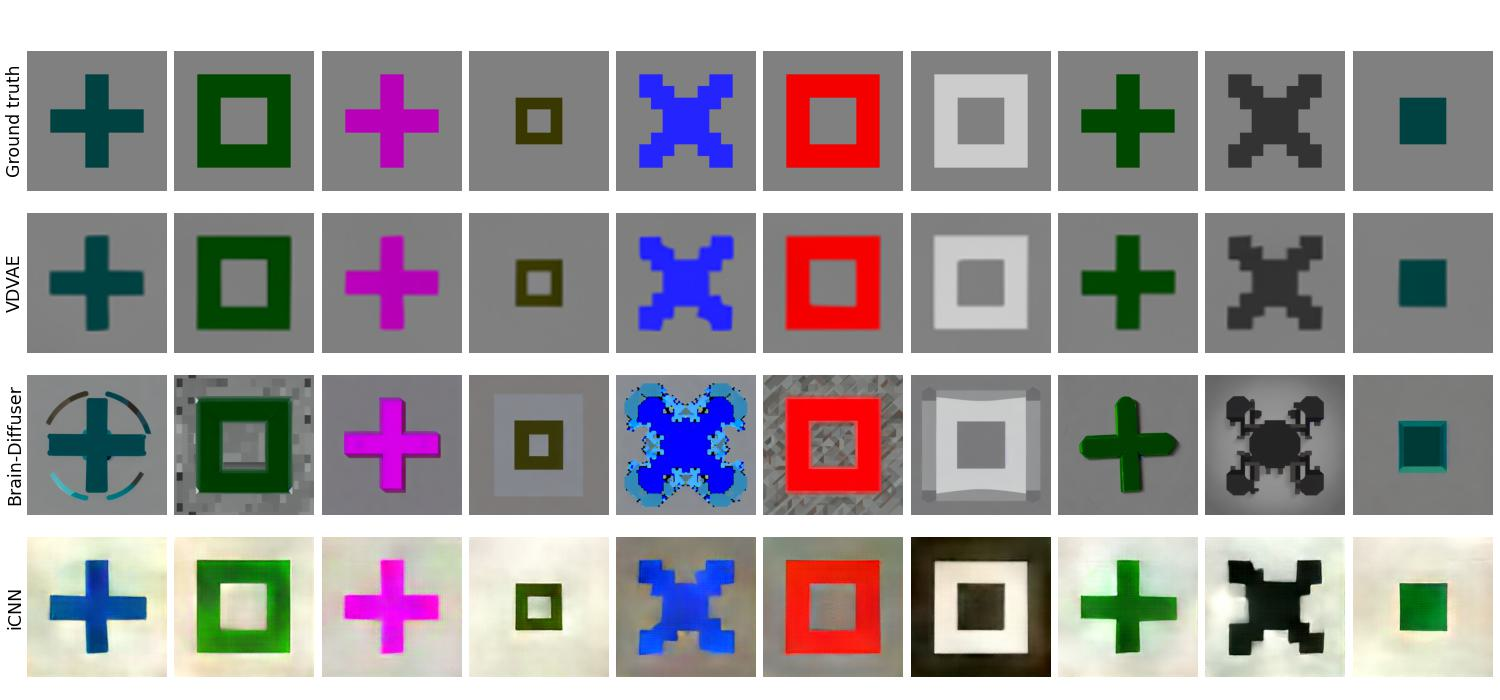
\includegraphics[width=1\textwidth]{plots/baseline_qual_true_recon_art.JPEG}
    \caption[Recovery check for artificial shapes]{Recovery check for artificial shapes. \rOne{The top row depicts the ground truth image. Each following row depicts the reconstruction with true features with the algorithm named on the left side. Note that the VDVAE is only a part of the whole Brain-Diffuser algorithm.}}\label{fig:baselinetruerecon_art}
\end{figure}

% Small Evaluation of the True-Feature Reconstruction

\section{Evaluation metrics}
%% Regression Criteria
% Profile Correlation
% Pattern Correlation
% Pairwise Identification Accuracy

It is possible to evaluate both stages of the reconstruction algorithms (the \rOne{translation} and the reconstruction). The results of the regressions are used to evaluate the \rOne{translation} part of the algorithms and the final reconstructed images are examined to evaluate the reconstruction part of the algorithms. \rOne{Each presentation of an image for a subject is treated as an independent sample. The data from the different subjects is interpreted as a unit for replicating the experiment to investigate the robustness of the results. Thus the data will not be pooled across the subjects and statistical tests will not be executed.} Thus, even though quantitative metrics are computed, they will be evaluated in a rather qualitative way by referring plots and interpreting the results.


\subsection{Measuring \rOne{translation} performance}
\rOne{To evaluate the translation performance, pairwise identification accuracy will be used}. The pairwise identification accuracy is a metric frequently used to determine the feature prediction in reconstruction algorithms~\cite{shirakawaSpuriousReconstructionBrain2024}. 
The pairwise identification accuracy measures whether a predicted feature vector is more similar to the true feature than the other predicted vectors. For a feature vector $i$, it is defined as:


\[ % Only for image i
\text{PairwiseIDAcc}_i \coloneq \frac{1}{n-1} \sum_{\substack{j=1 \\ j \neq i}}^{n} \mathbb{I} \left(  \text{sim}\left(\hat{y}_{i}, y_{i}\right)  > \text{sim}\left(\hat{y}_{j}, y_{i} \right) \right)
\]
\noindent{}\rTwo{where \( y_{i} \) represents the true feature vector for the \( i \)-th sample, \( \hat{y}_{i} \) represents the predicted feature vector for the \( i \)-th sample, \( \text{sim}\left( \cdot, \cdot \right) \) denotes an arbitrary distance metric for vectors and \( \mathbb{I}(\cdot) \) is the indicator function, which equals 1 if the condition inside is true and 0 otherwise.} The \rOne{similarity} metric can be freely chosen, in this work, the cosine \rOne{similarity} is used, since the high dimensionality negatively affects the euclidean distance~\cite{koppen2000curse}. The cosine \rOne{similarity} between to vectors \textbf{a} and \textbf{b} is calculated as follows:

\[
\text{cosine\_sim}(a, b) \coloneq \frac{a \cdot b}{\|a\| \, \|b\|}
\]

\noindent{}If a feature vector cannot be predicted from brain activity, one would expect the pairwise identification accuracy to be 0.5, since it will be a matter of chance whether any other vector is  more or less similar to the true feature than the actually predicted feature vector. In order to compute the Pairwise Identification Accuracy, for the different \rOne{translators} of the iCNN and the Brain-Diffuser, the corresponding multidimensional feature vectors are reshaped to a one-dimensional vector to be able to compute the vector similarity between layers (for example the convolutional layers of the VGG19 are multidimensional). \rOne{The pairwise identification may be abbreviated as ID Accuracy in the following}. 


\subsection{Measuring reconstruction performance}

The final results of the reconstruction algorithms can in turn be analysed both qualitatively and quantitatively. Different metrics can be used to compare the ground truth images and the reconstructed images on a quantitative level~\cite{ozcelikNaturalSceneReconstruction2023}. On the one hand, the metrics can focus on the low-level features of an image (e.g.\ structure and colour); on the other hand, there are metrics that compare the high-level features of the images (i.e.\ the semantic meaning). For an appropriate judgement on the overall quality of a reconstruction, it is important to consider both the low-level and high-level features (a reconstructed image that has the correct outlines but completely ignores the semantic concepts is just as bad as an image in which the meaning has been correctly captured but the position and position of the objects in the image are incorrectly represented).

In this work, the PixelCorrelation is used as a low-level metric~\cite{shenDeepImageReconstruction2019,ozcelikNaturalSceneReconstruction2023}. In this method, the reconstructed images and the ground truth image are first reshaped into a one-dimensional vector and the correlation between the two is then calculated. The expected value for random reconstructions would be $r=0$. \rOne{The PixelCorrelation may be abbreviated with PixCorr in some plots}.

\rOne{CLIP-accuracy measures the semantic (high-level) similarity between reconstructed images and ground truth images by embedding both into a shared semantic feature space using a CLIP Vision encoder~\cite{radfordLearningTransferableVisual2021}. To align with the evaluation methodology of Brain-Diffuser~\cite{ozcelikNaturalSceneReconstruction2023} and ensure comparability with their results, this study adopts the same approach. This metric quantifies how frequently the embedded semantic features of correctly matched image pairs (each reconstructed image with its corresponding ground truth) show higher correlation compared to incorrectly matched pairs (a reconstructed image with a non-corresponding ground truth). Thus this metric is very similar to the pairwise identification accuracy that was described above, only that it is comparing the results in the CLIP feature space. The random chance-level baseline for this metric is again 0.5. \rTwo{To} make the CLIP-accuracy results more directly comparable in scale to other metrics used in this thesis, the random baseline value of 0.5 is subtracted from the raw accuracy scores. Consequently, the adjusted CLIP-accuracy presented here has a random-chance baseline of 0 and a theoretical maximum of 0.5. The CLIP-accuracy may be abbreviated with CLIP-acc in some plots.}

In addition to the low-level and high-level differences, a third quantiative metric is used in this work to test the reconstruction performance. Since the natural human judgement about the similarity of images is based on several visual attributes that integrate low-level features with high-level features~\cite{sundaramWhenDoesPerceptual2024}, DreamSim~\cite{fuDreamSimLearningNew2023} was developed to get closer to the natural judgement about the similarity of images. DreamSim combines various image features and has been fine-tuned with human judgement to better estimate the ``mid-level'' similarity between images. To calculate the similarity between two images, the cosine-similarity (i.e.\ 1\@ $-$\@ cosine distance) between the DreamSim embedding vector of the ground truth and the predicted image is calculated. In a random reconstruction, the cosine similarity would be 0 (the feature vectors are be orthogonal to each other). \rOne{Note that the cosine distance may be abbreviated as cos\_dist in some plots.}

Since even the DreamSim metric is not perfect for comparing the similarity of images, and since judgments of quality may vary from person to person, the differences are also described qualitatively. Individual examples of the actual reconstructed images are shown and compared to the ground truth images for each test condition tested in this paper.

\section{Baseline results}
In order to validate the reconstruction algorithms used in this work, the results of the two algorithms are presented below. No other changes were made to the input datasets or the method, so the results can be used as a baseline for comparison with the further results of the following experiments.

\subsection{\rOne{Translation} results}
\rOne{Figure~\ref{fig:baselinetranslator} shows the results for the \rThree{translator}. The mean values over all 50 (natural test images) or 40 (artificial images) test samples are shown. The error bars are the standard errors. From now on, all error bars in this study will be standard errors over the 50 (or 40 respectively) test images unless reported otherwise. All mean values for all participants are clearly above the random probability of 0.5. Thus, for both the Brain-Diffuser and iCNN, the \rOne{translators} have the ability to predict the true features of the test images to some extent. The performance is also relatively constant across the different subjects, with the significantly larger differences being found between the different \rOne{translator} modules. In particular, for the CLIP Text features, the identification accuracy is very high at 0.892 on average and is already close to the upper limit of 1.0. \rThree{For the artificial shapes,} a slightly different picture emerges in contrast to the natural test images. Here, \rOne{translator} has to generalise outside its training domain. All individual values are lower than with the natural test images. iCNN (from 0.831 to 0.782) and VDVAE (from 0.761 to 0.665) show only a comparatively small drop in performance. For the two CLIP \rOne{translator}, the difference to the natural test images is significantly greater (CLIP Vision falls from 0.777 to 0.54 and CLIP Text falls from 0.892 to 0.558). The identification accuracy for the CLIP \rOne{translators} is only just above the chance probability of 0.5 for the artificial test images.}

% In addition, the results aggregated over all 5 subjects for both types of test images are listed in Table~\ref{tab:baseline_translator}, with the standard deviation in parentheses.


\begin{figure}[ht]
    \centering
    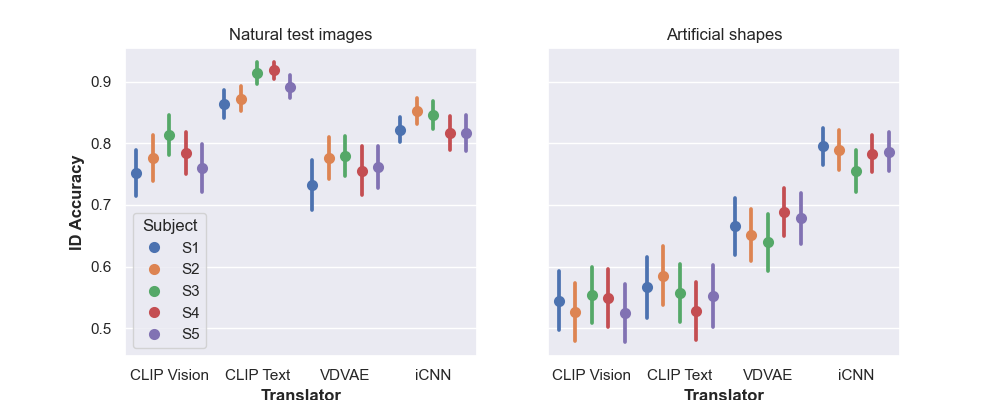
\includegraphics[width=1\textwidth]{plots/baseline_translator.png}
    \caption[Translator performance baseline]{\rOne{Translator} performance for the Brain-Diffuser and iCNN on natural test images and artificial shapes. \rOne{The identification accuracy of all four translators (the three translators for VDVAE, CLIP Text and CLIP Vision from the Brain-Diffuser and the translator for the iCNN) is depicted for each of the five subjects. The standard error across all test samples is depicted in the error bars.}}\label{fig:baselinetranslator}
\end{figure}


% \begin{figure}[ht]
%     \centering
%     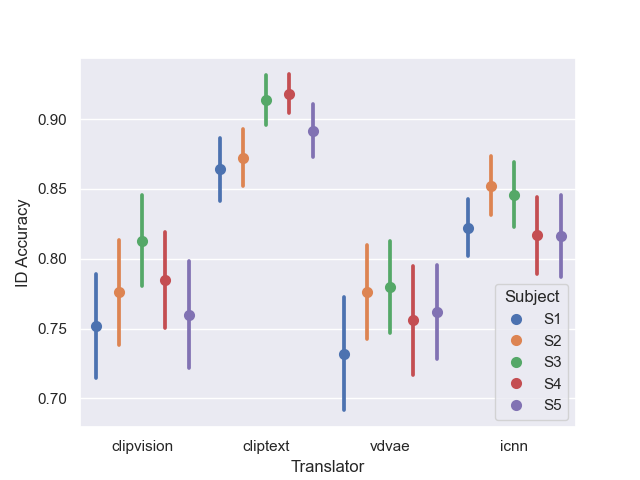
\includegraphics[width=0.6\textwidth]{plots/baseline_translator_test.png}
%     \caption[Translator performance natural test images baseline]{\rOne{Translator} performance for the Brain-Diffuser and iCNN on natural test images. \rOne{The identification accuracy of all four translators (the three translators for VDVAE, CLIP Text and CLIP Vision from the Brain-Diffuser and the translator for the iCNN) is depicted for each of the five subjects. The standard error across all test samples is depicted in the error bars.}}\label{fig:baselinetranslatortest}
% \end{figure}

% \begin{figure}[ht]
%     \centering
%     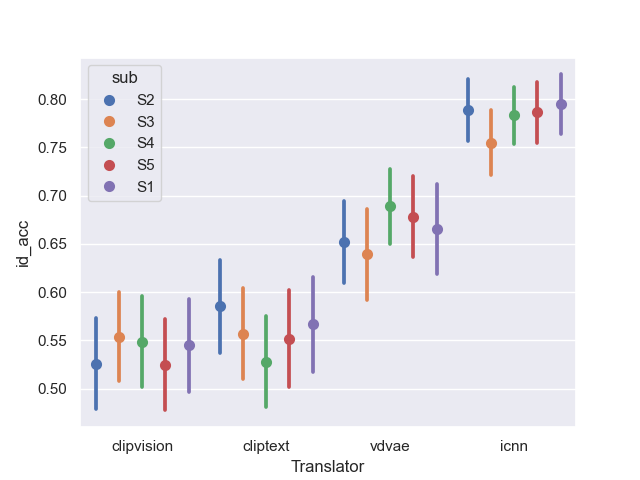
\includegraphics[width=0.6\textwidth]{plots/baseline_translator_art.png}
%     \caption[Translator performance artificial shapes baseline]{\rOne{Translator} performance for the Brain-Diffuser and iCNN on artificial shapes. \rOne{The identification accuracy of all four translators (the three translators for VDVAE, CLIP Text and CLIP Vision from the Brain-Diffuser and the translator for the iCNN) is depicted for each of the five subjects. The standard error across all test samples is depicted in the error bars.}}\label{fig:baselinetranslatorart}
% \end{figure}

% \begin{table}[ht]
%     \centering
% \begin{tabular}{lllll}
\toprule
 & clipvision & cliptext & vdvae & icnn \\
test images &  &  &  &  \\
\midrule
natural & 0.777 (.024) & 0.892 (.024) & 0.761 (.019) & 0.831 (.017) \\
artificial & 0.54 (.013) & 0.558 (.021) & 0.665 (.02) & 0.782 (.016) \\
\bottomrule
\end{tabular}

% \caption{A nice table.}\label{tab:baseline_translator}
% \end{table}


\subsection{Reconstruction results}
\rOne{Ten of the reconstructed images are shown for the natural test images in Figure~\ref{fig:baselinerecontestqual} 
As with the true-feature reconstruction, both the intermediate result of the VDVAE and the overall result are shown here for the Brain-Diffuser algorithm. The VDVAE and iCNN tend to produce blurred outlines, while the Brain-Diffuser algorithm usually creates photorealistic objects. For the natural test images, the VDVAE and iCNN usually \rOne{translate} the outlines approximately correctly. For example, the ball produces a round object in front of a neutral background and the goldfish is reconstructed as a red, elongated object in front of a dark background. The VDVAE produced artefacts for the aeroplane, which could be the result of clipping in the prediction (the predicted values of the features are too high or too low and distort the pixel value). All in all, the results of the VDVAE and iCNN are comparable. The full Brain-Diffuser algorithm is designed to add semantic information to the results of the VDVAE and incorporate this into a photorealistic image with the versatile diffusion process. In the case of natural test images, it looks as if this is at least partially successful: the images that represent living beings (bat, llama, goldfish or orca) also look as if something alive is to be represented in the reconstructed version (even if the exact animal cannot be recognised). Likewise, the inanimate objects (e.g.\ the hat, the surgical instrument or the umbrella) are also reconstructed in a comparatively neutral way. Even the snowmobile looks like a vehicle (with handlebars and wheels) after reconstruction. Only in the case of the aircraft is the interpretation difficult, but this may also be due to the faulty result of the VDVAE.\@ The reconstructed artificial shapes are displayed in Figure~\ref{fig:baselinereconartqual}. The figure follows the same structure as before.The VDVAE and iCNN are again largely able to reconstruct the correct shapes for the here. Only the shape `X' cannot be reconstructed very well. As the results of the \rOne{translator} already indicated, the final Brain-Diffuser result for the artificial shapes is far from perfect. Here, too, photorealistic images are usually generated. The shapes are often well adopted by the VDVAE and then converted into a photorealistic image with false details hallucinated by the diffusion algorithm (for example, in the image with the purple cross on a person can be seen).}

The plot in Figure~\ref{fig:baselinereconquant} shows the results of the quantitative evaluation of the image reconstruction for the individual subjects. As with the \rOne{translators}, the error bars are the standard errors. The three previously described measurement parameters, PixelCorrelation, DreamSim-distance and CLIP-accuracy, are shown for the iCNN and Brain-Diffuser (bd) algorithms. For the natural test images, \rOne{there is only a slight difference between iCNN and Brain-Diffuser in terms of DreamSim (iCNN has a slightly higher DreamSim than Brain-Diffuser)}. In terms of CLIP accuracy, however, the reconstructions of the Brain-Diffuser show consistently higher performance than the iCNN.\@ The difference in the pixel correlation is not as visible in the graphic, but it appears that the iCNN consistently achieves higher results in this low-level metric than the Brain-Diffuser. \rThree{For the artificial shapes}, as with the \rOne{translator}, the results are \rOne{in general} less accurate than for the natural images. The iCNN now clearly performs better than the Brain-Diffuser in terms of both the DreamSim-distance and the pixel correlation. For the CLIP accuracy \rOne{(where before the Brain-Diffuser performed better than iCNN)}, there is no longer any \rOne{visible} difference between the two algorithms, and the results are very close to the random probability of 0.5. 


\begin{figure}[ht]
    \centering
    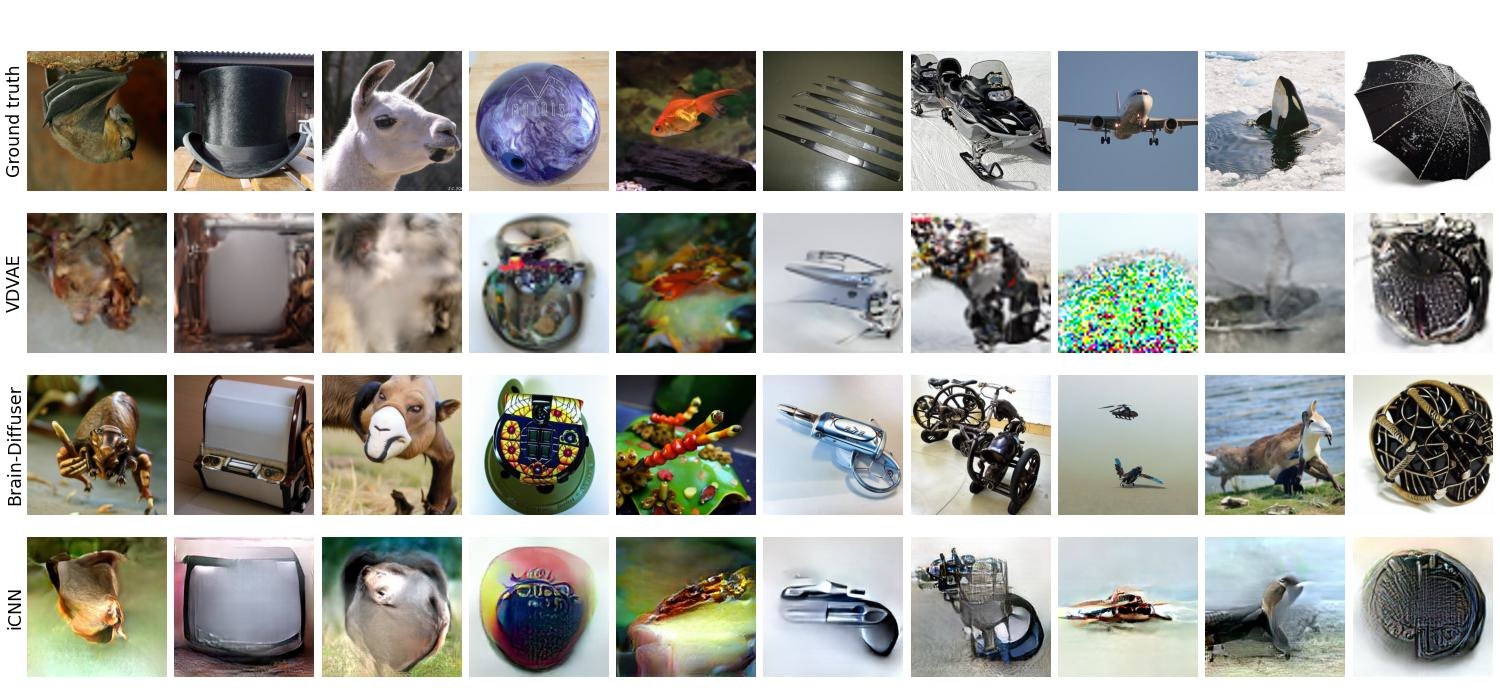
\includegraphics[width=1\textwidth]{plots/baseline_qual_recon_test.JPEG}
    \caption[Reconstructed images for iCNN and Brain-Diffuser on natural test images]{Qualitative results of iCNN and Brain-Diffuser on natural test images. \rOne{The top row depicts the ground truth image. Each following row depicts the reconstruction from the predicted features with the algorithm named on the left side. Note that the VDVAE is only a part of the whole Brain-Diffuser algorithm.}}\label{fig:baselinerecontestqual}
\end{figure}

\begin{figure}[ht]
    \centering
    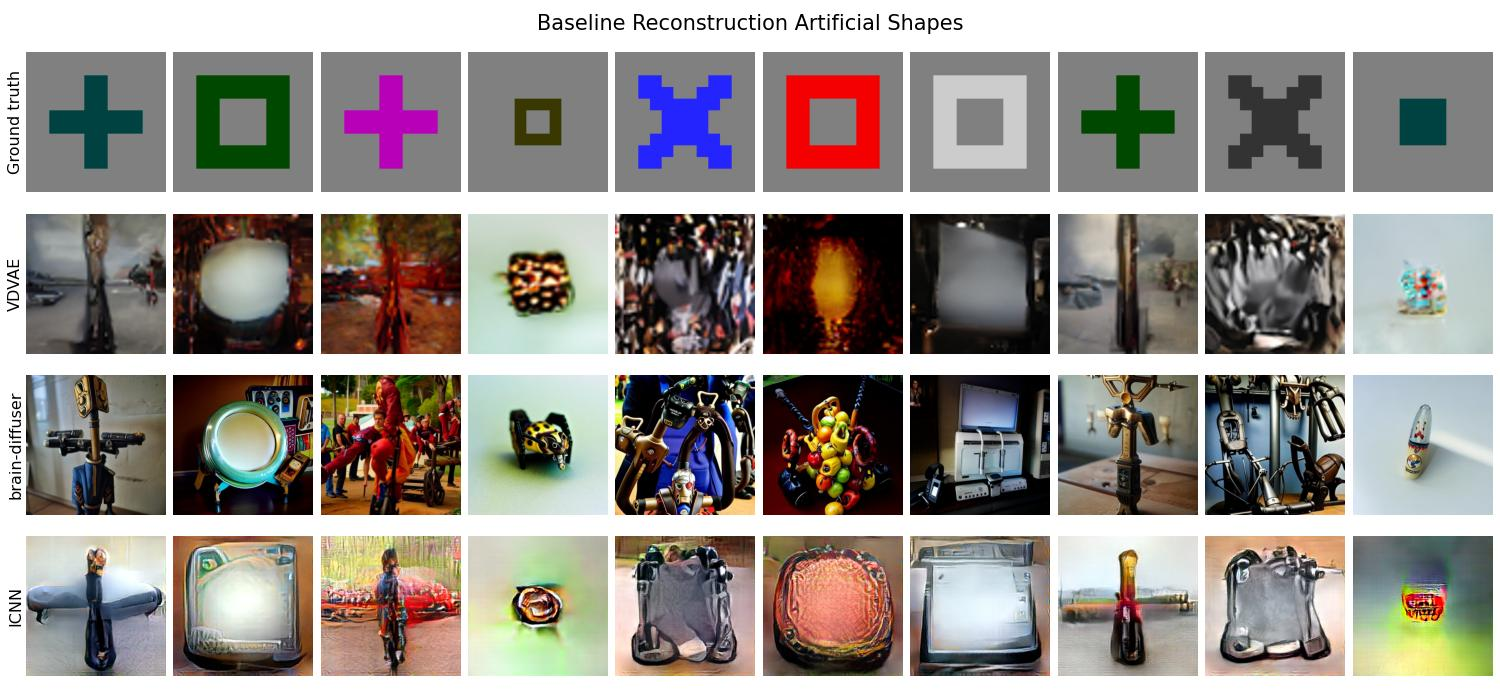
\includegraphics[width=1\textwidth]{plots/baseline_qual_recon_art.JPEG}
    \caption[Reconstructed images for iCNN and Brain-Diffuser on artificial shapes]{Qualitative results of iCNN and Brain-Diffuser on artificial shapes. \rOne{The top row depicts the ground truth image. Each following row depicts the reconstruction from the predicted features with the algorithm named on the left side. Note that the VDVAE is only a part of the whole Brain-Diffuser algorithm.}}\label{fig:baselinereconartqual}
\end{figure}


\begin{figure}[ht]
    \centering
    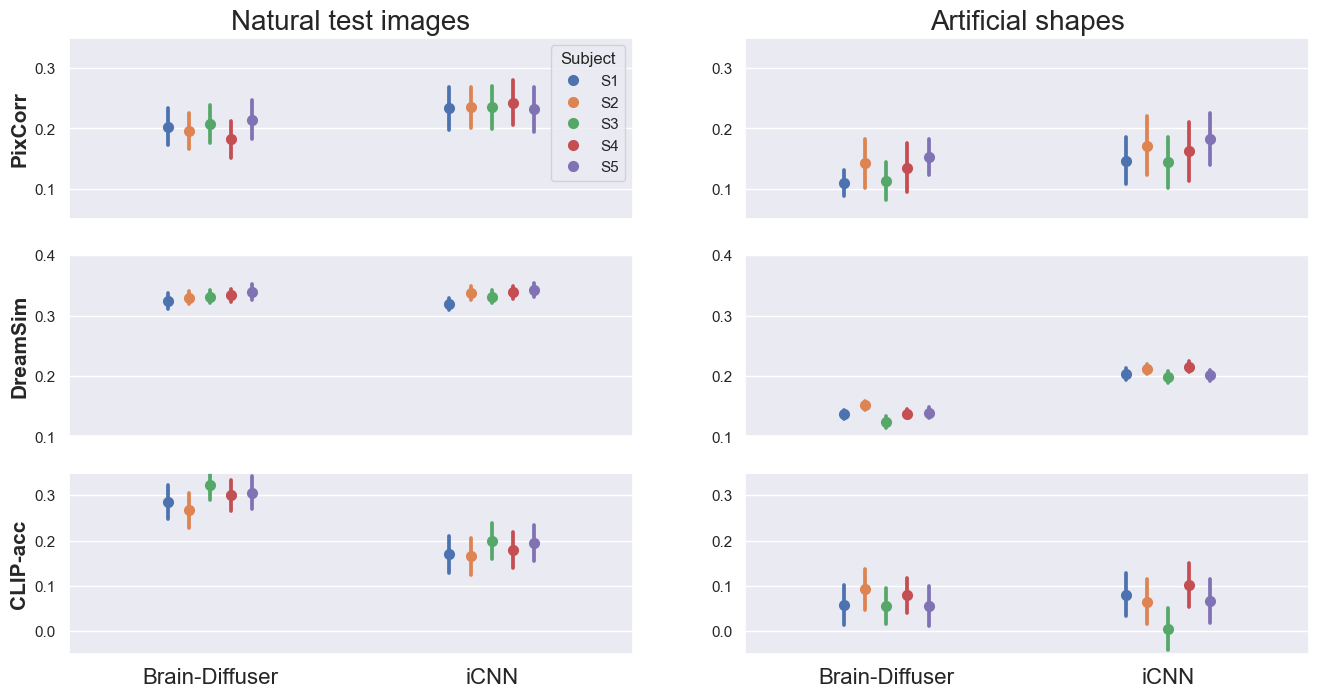
\includegraphics[width=1\textwidth]{plots/baseline_reconstruction.png}
    \caption[Reconstruction performance baseline]{Reconstruction performance of iCNN and Brain-Diffuser. \rOne{For each of the five subjects, the three reconstruction criteria (PixelCorrelation, DreamSim and CLIP-accuracy) are displayed for both the Brain-Diffuser and iCNN algorithm. The errorbars are computed as the standard error across all the test samples.}}\label{fig:baselinereconquant}
\end{figure}

% \begin{figure}[ht]
%     \centering
%     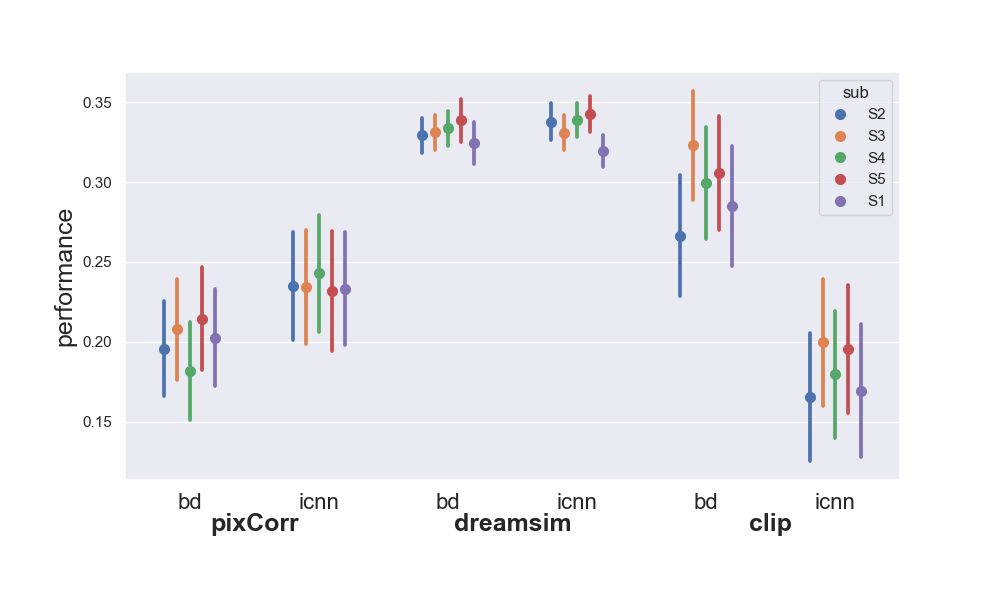
\includegraphics[width=0.8\textwidth]{plots/baseline_reconstruction_test.png}
%     \caption[Reconstruction performance natural test images baseline]{Reconstruction performance of iCNN and Brain-Diffuser on natural test images. \rOne{For each of the five subjects, the three reconstruction criteria (PixelCorrelation, DreamSim and CLIP-accuracy) are displayed for both the Brain-Diffuser and iCNN algorithm. The errorbars are computed as the standard error across all the test samples.}}\label{fig:baselinerecontestquant}
% \end{figure}

% \begin{figure}[ht]
%     \centering
%     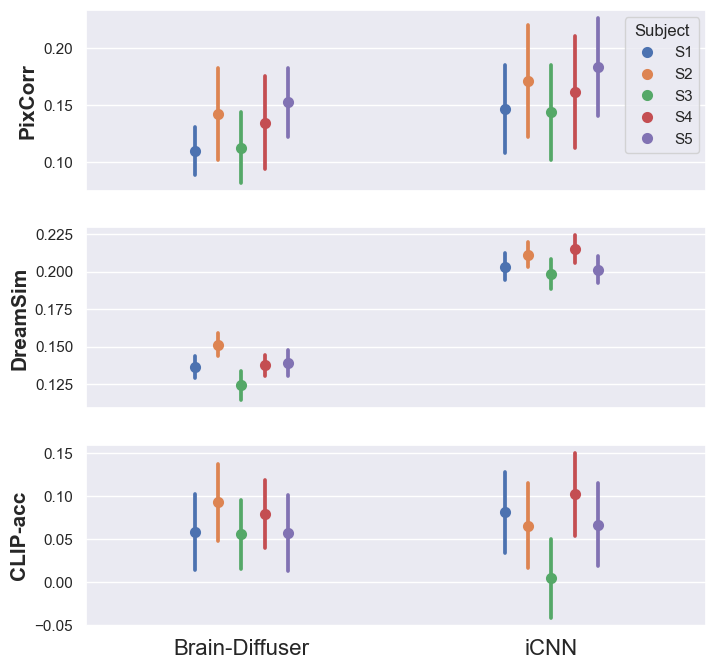
\includegraphics[width=0.8\textwidth]{plots/baseline_reconstruction_art.png}
%     \caption[Reconstruction performance artificial shapes baseline]{Reconstruction performance of iCNN and Brain-Diffuser on artificial shapes. \rOne{For each of the five subjects, the three reconstruction criteria (PixelCorrelation, DreamSim and CLIP-accuracy) are displayed for both the Brain-Diffuser and iCNN algorithm. The errorbars are computed as the standard error across all the test samples.}}\label{fig:baselinereconartquan}
% \end{figure}

% \begin{table}[ht]
%     \centering
% \begin{tabular}{lllll}
\toprule
 &   & pixCorr & dreamsim & clip \\
test images & algorithm &  &  &  \\
\midrule
\multirow[t]{2}{*}{natural} & icnn & 0.235 (.004) & 0.334 (.009) & 0.682 (.015) \\
 & bd & 0.201 (.013) & 0.332 (.005) & 0.796 (.021) \\
\cline{1-5}
\multirow[t]{2}{*}{artificial} & icnn & 0.161 (.017) & 0.206 (.007) & 0.564 (.036) \\
 & bd & 0.13 (.019) & 0.138 (.01) & 0.568 (.017) \\
\cline{1-5}
\bottomrule
\end{tabular}

% \caption{A nice table.}\label{tab:baseline_reconstruction}
% \end{table}

\subsection{Conclusion}
The effectiveness of the two algorithms, Brain-Diffuser and iCNN, could be validated with the Deeprecon data set. It was shown that the \rOne{translator} modules of the algorithms were able to predict the features from the brain activity well above the random probability. Furthermore, it was shown that the reconstructed images also show strong similarities to the ground-truth images, so it is possible to a certain degree to reconstruct seen images from brain activity using the mentioned algorithms. The reconstructed images also look qualitatively similar to those in the relevant literature (see~\cite{shenDeepImageReconstruction2019, shirakawaSpuriousReconstructionBrain2024, ozcelikNaturalSceneReconstruction2023}).
In contrast to the original study, the Brain-Diffuser was evaluated with the Deeprecon dataset and not the NSD dataset. As already described, there is a partial overlap of semantic concepts between the training and the test dataset in the NSD dataset. Accordingly, the results of the Brain-Diffuser in our validation are worse than for the original author~\cite{ozcelikNaturalSceneReconstruction2023}. With our data, the Brain-Diffuser algorithm achieves a PixelCorrelation of 0.201 (0.305 for the original authors) and a CLIP-accuracy of 0.796 (0.925 for the original authors). In particular, the high difference in CLIP accuracy is to be expected, since the semantic overlap between training and test data in the NSD dataset enables the semantic categories to be learned. Thus, the CLIP \rOne{translators} do not need to learn a regression on the complete possible CLIP space, but only needs to perform a classification (generalisation over unknown classes is not fully possible). 
Nevertheless, our results with the Deeprecon data set showed that at least parts of the semantic meaning of the images could be captured (e.g.\ living vs.\ inanimate objects). At least for the natural test data, it has been shown that the iCNN algorithm is better able to reconstruct the low-level structure of an image (difference of PixelCorrelation), while the Brain-Diffuser is better able to recognise high-level concepts (difference of CLIP-accuracy). 
The artificial shapes were consistently  reconstructed worse than the natural test images. This indicates the additional difficulty of out-of-distribution generalisation. Compared to Brain-Diffuser, the iCNN algorithm has lost significantly less in its reconstruction quality. This can be explained by the fact that iCNN is less dependent on learned categories than Brain-Diffuser and thus generalises more easily. The Brain-Diffuser shows the significantly poorer generalisation described by Shirakawa et.\ al.~\cite{shirakawaSpuriousReconstructionBrain2024} The main cause for this is described as output dimension collapse: the \rOne{translator} modules have not been trained with sufficiently diverse data and therefore map to the semantic space known from the training, in which potential (previously unknown) dimensions in the test data set cannot be mapped. To improve the generalisation of the algorithms, it is therefore necessary to have more diverse data in the training set to enable regression into dimensions not present in the training. In the following, we will thus investigate in different experiments what influence the diversity of the training data has on reconstruction and out-of-distribution generalisation, and how the diversity of existing data sets can presumably be increased. 